% Created 2023-03-31 Fri 18:36
% Intended LaTeX compiler: pdflatex
\documentclass[11pt]{article}
\usepackage[utf8]{inputenc}
\usepackage[T1]{fontenc}
\usepackage{graphicx}
\usepackage{longtable}
\usepackage{wrapfig}
\usepackage{rotating}
\usepackage[normalem]{ulem}
\usepackage{amsmath}
\usepackage{amssymb}
\usepackage{capt-of}
\usepackage{hyperref}
\author{Yusheng Zhao}
\date{\today}
\title{Homework 2}
\hypersetup{
 pdfauthor={Yusheng Zhao},
 pdftitle={Homework 2},
 pdfkeywords={},
 pdfsubject={},
 pdfcreator={Emacs 28.2 (Org mode 9.6.1)}, 
 pdflang={English}}
\begin{document}

\maketitle
\tableofcontents


\section{Problem 1}
\label{sec:org5931637}
\subsection{A}
\label{sec:org1ee1d7a}
\(F(x) = - \frac{\partial U(x)}{\partial x} = -(x-1)\), at \(t=0\), \(x=0\) so \(F= 1\).
\subsection{B}
\label{sec:orgb6f50ab}
According to the velocity Verlet algorithm, we know
\[\vec{x}(t+\delta t) = \vec{x}(t) + \delta t \vec{v}(t) + \frac{1}{2} \delta t^2 \vec{a}(t)\]
and
\[\vec{v}(t + \delta t) = \vec{v}(t) + \frac{1}{2}\delta t [\vec{a}(t) + \vec{a}(t+\delta t)]\]
with \(x(0)  = 0, v(0) = 0, a(0) = F(0)/m = 1\),
\[\vec{x}(\Delta t = 0.5)  = 1/8 \]
then,  \(a(\Delta t = 0.5) = -(1/8-1) = 7/8\)
\[ \vec{v}(\Delta t = 0.5) =  15/32\]
\subsection{C}
\label{sec:orgfdb1e6e}
We know \(E = \frac{1}{2}mv^2 + \frac{1}{2}(x-1)^2\), for \(t = 0\), \(E = 0.5\). For \(t = 0.5\), \(E = 225/2048 + 49/128 = 1009/2048 \approx 0.492675\)
\subsection{D}
\label{sec:org944e1db}
It was not conserved. This is because the time-step is not truly infinitesimal,
the updated velocity position are not truly accurate. Therefore, there will be
error in the energy calculated according to those values.

\section{Problem 2}
\label{sec:org6e0bdf5}
\subsection{A}
\label{sec:org5df4b88}
\begin{verbatim}
using CairoMakie
u612(x) = 4 * ((1/x^12) - (1/x^6))
u510(x) = 4 * ((1/x^10) - (1/x^5))
f = Figure()
ax = Axis(f[1, 1],
    title = "Lenord Jones Potential",
    xlabel = "r (units)",
    ylabel = "U(r)  (units)"
)
x = 1.0:0.001:6
u1 = u612.(x)
u2 = u510.(x)
lin612 = lines!(ax, x, u1,label="6-12 Potential")
lin510 = lines!(ax, x, u2,label="5-10 Potential")
axislegend()
save("p2.png",f)
\end{verbatim}

\subsection{B}
\label{sec:org710f742}
According to the plot, the potential energy mainly dies out around \(r = 2.5\).
Therefore, I would assign \(r_{u} = 2.5\) and \(r_{l} = 0.9* r_{u} = 2.25\). Then
the cutoff function \(S(r)\) will be introduced as
\begin{align}
    \begin{cases}
    S(r) = 1 ; r < r_{l} \\
    S(r) = \frac{(r_{u}-r)^2(r_{u}+2r-3r_{l})}{(r_{u}-r_{l})^3} ; r_{l} < r < r_{u} \\
    S(r) = 0; r > r_{u}
    \end{cases}
\end{align}
There was a typo in the slides.

\begin{center}
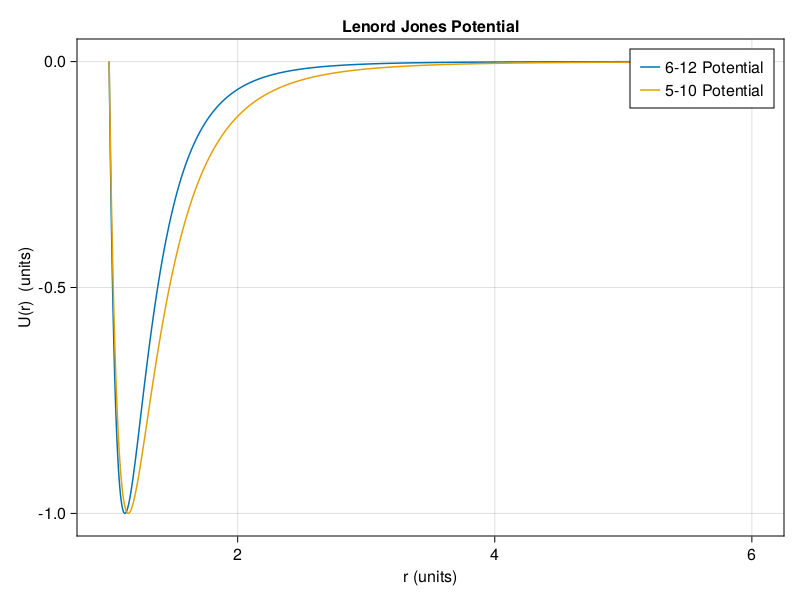
\includegraphics[width=.9\linewidth]{./p2.png}
\end{center}

\subsection{C}
\label{sec:org58d57d6}
\begin{verbatim}
using CairoMakie
function sr(r::T,rl::T,ru::T) where T
    if r < rl
        return one(r)
    elseif r > ru
        return zero(r)
    else
        return (ru-r)^2 * (ru + 2*r - 3*rl) / (ru-rl)^3
    end
end
u612(x) = 4 * ((1/x^12) - (1/x^6))
u510(x) = 4 * ((1/x^10) - (1/x^5))
f = Figure()
ax = Axis(f[1, 1],
    title = "Shifted Lenord Jones Potential",
    xlabel = "r (units)",
    ylabel = "U(r)*S(r)  (units)"
)
x = 1.0:0.001:6
ru = 2.5
u1 = u612.(x) .* sr.(x, 0.9*ru, ru)
u2 = u510.(x) .* sr.(x, 0.9*ru, ru)
lin612 = lines!(ax, x, u1,label="Shifted 6-12 Potential")
lin510 = lines!(ax, x, u2,label="Shifted 5-10 Potential")
axislegend()
save("p2_shifted.png",f)

\end{verbatim}
\begin{center}
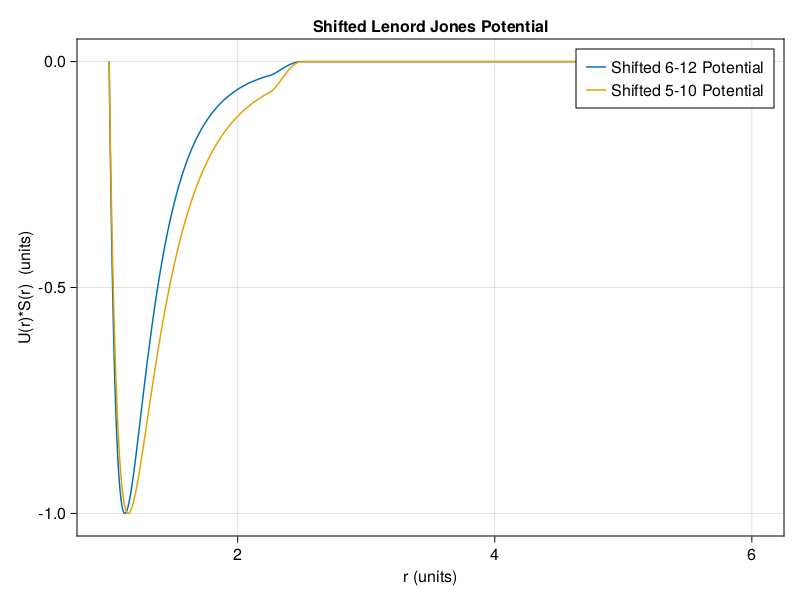
\includegraphics[width=.9\linewidth]{./p2_shifted.png}
\end{center} There should not be any efficiency difference since both
functions are turned off at the same position \(r\). In terms of accuracy, I guess
\(5-10\) L-J potential will win.
\section{Problem 3}
\label{sec:org82b63c1}
In partition function, the probability of a state is proportional to
\(e^{KE/k_BT}\). If you want the probability to stay the same, you need
\(KE_{inst}/(k_{B} T_{inst}) = KE_{target}/k_{B}T_{Target}\) therefore,
\(v_{inst}/v_{target} = \sqrt{\frac{T_{inst}}{T_{target}}}\)

\section{Problem 4}
\label{sec:orgf79e9c3}
\begin{verbatim}
begin
    using Random, Distributions, Plots
    n_trials = 10000
    samples = rand(Uniform(-1,1),(2,n_trials))
    sums = zeros(Float64,n_trials+1)
    for ctr in 1:n_trials
        x,y = samples[:,ctr]
        if x^2 + y^2 <= 1
            sums[ctr+1] = sums[ctr] + 1.0
        else
            sums[ctr+1] = sums[ctr]
        end
    end
    #we are essentially estimating the area
    sums ./= 1:n_trials+1
    sums .*= 4
    plot(1:length(sums), sums,xlabel="Steps",ylabel="Estimation",title="MC steps vs estimated value")
    savefig("mc.png")
    println("Estimation of pi is: $(sums[end])")
end
\end{verbatim}

I esimated \(\pi\) to be \(3.12888711128887\). Please see the plot below.

\begin{center}
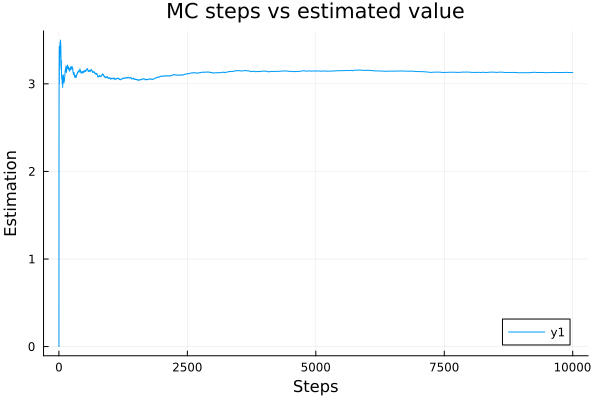
\includegraphics[width=.9\linewidth]{./mc.png}
\end{center}
\end{document}